\chapter{Lab 2: Kalman filter}

\section{Main steps}

\begin{enumerate}
    \item TODO
\end{enumerate}

\section{State space model}

\begin{figure}[H]
    \centering
    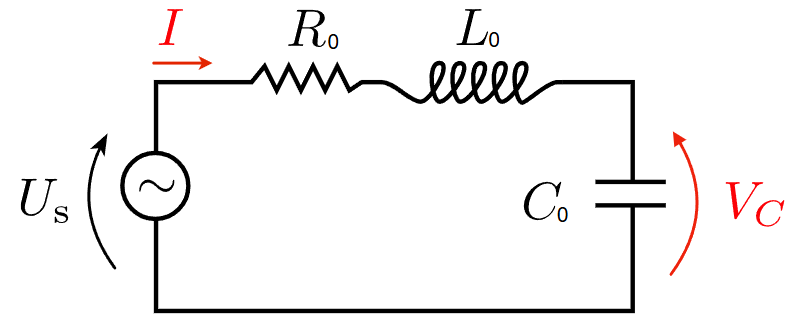
\includegraphics[width=0.8\textwidth]{pic/RLC.png}
    \caption{Studied RLC circuit}
    \label{fig:RLC_circuit}
\end{figure}

The studied system is the RLC circuit shown in Fig \ref{fig:RLC_circuit}. A set of equations can be derived using Kirchhoff's laws:

\begin{gather}
    u_s(t) = R_0\, i(t) + L_0 \frac{d i(t)}{dt} + \frac{1}{C_0} \int i(t)\,dt\\
    v_C(t) = \frac{1}{C_0} \int i(t)\,dt
\end{gather}

By substituting the second equation into the first one, we obtain:

\begin{equation}
    u_s(t) = R_0\, i(t) + L_0 \frac{d i(t)}{dt} + v_C(t)
\end{equation}

To get to the continuous-time state space representation of this circuit, we need to define the input of the system as $u_s(t)$, its output as $v_C(t)$ and the state vector as:

\begin{equation}
    x(t) = \begin{bmatrix} x_1(t) \\ x_2(t) \end{bmatrix} = \begin{bmatrix} v_C(t) \\ i(t) \end{bmatrix}
\end{equation}

Which finally leads to:

\begin{gather}
    \frac{d}{dt} \begin{bmatrix} x_1(t) \\ x_2(t) \end{bmatrix} = \begin{bmatrix} 0 & \frac{1}{C_0} \\ -\frac{1}{L_0} & -\frac{R_0}{L_0} \end{bmatrix} \begin{bmatrix} x_1(t) \\ x_2(t) \end{bmatrix} + \begin{bmatrix} 0 \\ \frac{1}{L_0} \end{bmatrix} u_s(t)\\
    y(t) = \begin{bmatrix} 1 & 0 \end{bmatrix} \begin{bmatrix} x_1(t) \\ x_2(t) \end{bmatrix}
\end{gather}

\begin{equation}
    \Leftrightarrow \hspace{1cm} A_c = \begin{bmatrix} 0 & \frac{1}{C_0} \\ -\frac{1}{L_0} & -\frac{R_0}{L_0} \end{bmatrix}, \hspace{1cm} B_c = \begin{bmatrix} 0 \\ \frac{1}{L_0} \end{bmatrix}, \hspace{1cm} C_c = \begin{bmatrix} 1 & 0 \end{bmatrix}, \hspace{1cm} D_c = 0
\end{equation}
